\begin{center}
    \textbf{--------- Lezione 8 - 8 aprile 2021 ---------}
\end{center}

\section{Introduzione al riconoscimento di attività}
L'activity recognition si colloca nel context-awareness, dove le applicazioni sono consce del contesto. 

Ci sono diversi esempi di uso di contesto nelle applicazioni mobili:
\begin{itemize}
    \item app che ricorda di scendere alla fermata del tram giusta
    \item app che suggerisce la strada in base al traffico attuale (tipo waze)
    \item app che ricorda di prendere l'ombrello prima di uscire di casa quando piove (capisce quando l'utente è a casa e che c'è un tempo sfavorevole)
\end{itemize} 

Uno dei più importanti aspetti dell'analisi del contesto è capire cosa fa l'utente, attraverso le tecnologie sensoristiche, e questo prende il nome di activity recognition. 

Le attività svolte dall'utente possono essere:
\begin{itemize}
    \item fisiche: attività di basso livello, relative a specifici movimenti, che vengono monitorate con dispositivi mobili o dispositivi wearable. Sono attività come correre, camminare, pedalare, ecc. 
    \item quotidiane: attività di alto livello che possono essere monitorate tramite sensori ambientali (es: smart-home). Sono attività come mangiare, cucinare, dormire, ecc.
\end{itemize}

Ci sono diverse soluzioni commerciali che monitorano le nostre attività e ci sono diversi servizi con le relative app che le mostrano, ad esempio il monitoraggio dello stile di vita, la qualità del sonno, il riconoscimento di attività in base ai luoghi visitati, ecc..

Sia Android che iOS mettono a disposizione delle API per riconoscere l'attività svolta dall'utente e possono essere usate per creare app che si adattano all'attività svolta dall'utente.

Il riconoscimento di questi sistemi non sempre è accurato, infatti una stessa attività può essere fatta da diversi utenti in modi differenti. 
C'è anche il problema che due attività diverse ma simili, vengono riconosciute come se fosse la stessa attività. 

\subsection{Riconoscimento}
I dispositivi mobili dispongono di diversi tipi di sensori che permettono di tracciare in modo continuo i movimenti fisici delle persone e che producono dati grezzi, cioè non ancora processati.
I dati vengono pre-processati e viene fatta pulizia.
Vengono passati ad un modello di riconoscimento, che può essere un sistema di AI, che capisce come mappare i dati pre-processati in attività e fornisce una predizione, cioè una distribuzione di probabilità (stai correndo al 80\%, stai camminando al 10\%, stai salendo le scale al 10\%). Viene poi fornito l'output del sistema, secondo l'attività più probabile. 
\vspace{1em}
\begin{figure}[!ht]
    \centering
    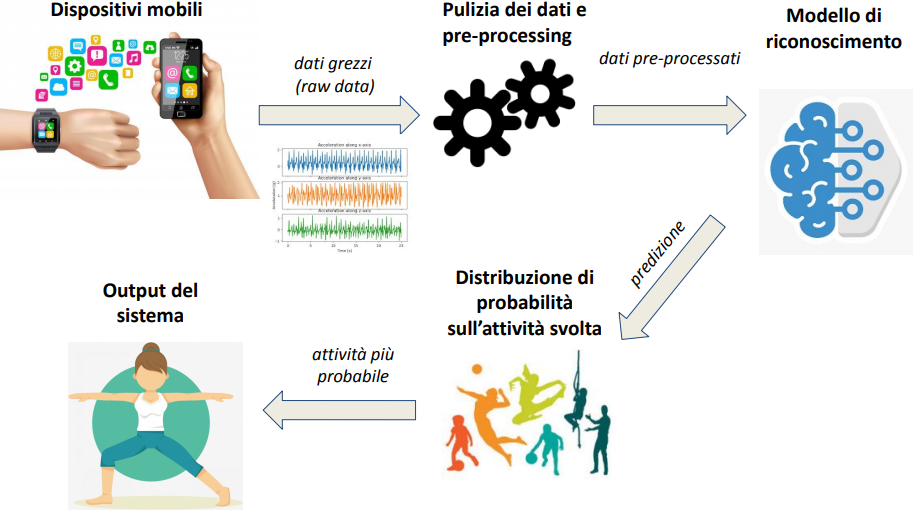
\includegraphics[width=.95\textwidth]{images/MobiDEV/6. activity recognition/processing.PNG}
    \caption{Riconoscimento}
    \label{fig:riconoscimento}
\end{figure}

%Il modello di riconoscimento deve essere costruito precedentemente. Si basa su un insieme di dati di sensori che sono stati ottenuti durante lo svolgimento di attività. Questi dati devono essere acquisiti prima della realizzazione del sistema di riconoscimento.

\section{Acquisizione dei dati grezzi di movimento dai dispositivi mobili}
I sensori inerziali, visti nella sezione \ref{subsubsec: sensori inerziali}, sono sensori che ci dicono qualcosa sui movimenti delle persone:
\begin{itemize}
    \item accelerometro: sui 3 assi ci dice la variazione di velocità che lo smartphone sta subendo. Si misura in $m/s^2$
    \item giroscopio: sui 3 assi indica la velocità angolare. Si misura in $grad/s$
    \item magnetometro: rileva la variazione nel campo magnetico. Si misura in $micro-Tesla$
\end{itemize} 
Ognuno di questi sensori produce dati su tutti e tre gli assi. 

Oltre ai sensori fisici, i sistemi operativi mettono a disposizione dei sensori virtuali, come ad esempio il contapassi. 

I sensori devono campionare una misurazione in intervalli e più la frequenza di campionamento è alta, più l'informazione è accurata, ma la computazione è più pesante e ci sono più dati da analizzare in fase di analisi. 

\section[Tecniche di machine learning per il riconoscimento di attività]{Tecniche di machine learning per il \\riconoscimento di attività}

Ci sono tecniche analitiche che permettono di analizzare il segnale e da cui possiamo capire cosa sta facendo una persona, ad esempio "se il valore dell'accelerometro sull'asse x è maggiore di 0.4 e il valore del giroscopio... allora l’utente sta correndo".

Le soluzioni analitiche hanno diversi limiti: 
\begin{itemize}
    \item ogni attività può essere svolta in modi molto diversi dalla stessa persona
    \item diverse persone possono svolgere la stessa attività in modo molto diverso
    \item attività diverse hanno dei pattern di movimento molto simili
    \item i dati dei sensori sono soggetti a rumore
\end{itemize} 

Il riconoscimento di attività fisiche si basa principalmente su tecniche di machine learning (ML), ovvero metodi statistici il cui scopo è trovare in modo automatico “pattern nascosti” nei dati.
Queste tecniche permettono di costruire un modello di attività che viene utilizzato per classificare i dati dei sensori.

Un problema su cui si basa activity recognition nel machine learning è la classificazione: dato un input X, vogliamo sapere a quale 
delle classi dell'insieme Y appartiene.
Nel ML, X ($\in \mathbb{R}^n$) è un vettore n-dimensionale che rappresenta il dato che vogliamo classificare.
Y è l'insieme delle attività, l'insieme delle possibili classi \{$y_1, y_2, ..., y_k$\}.
Ad ogni X corrisponde una classe $y_i$, ma non è nota.
Vogliamo trovare una funzione h(X) che approssimi al meglio il mapping tra elementi di $\mathbb{R}^n$ ed elementi di Y. Un sistema che implementa h è detto \textbf{classificatore}.
\begin{center}
    $h: \mathbb{R}^n \rightarrow Y$
\end{center}

Il ML non è una tecnica perfetta, ma un'approssimazione e si cerca che sia il più precisa possibile.

Ci sono diversi algoritmi di classificazione e sono divisi in categorie:
\begin{itemize}
    \item apprendimento supervisionato: si insegna con dei dati, in una fase precedente all'algoritmo, a riconoscere il mapping tra dati di sensori e attività. Una prima fase iniziale in cui vengono forniti (da parte del programmatore) degli esempi, e il sistema di ML sulla base di questi, impara ad associare i dati alle attività. Si ha un'etichetta associata all'attività dei dati
    \item apprendimento non supervisionato: abbiamo i dati iniziali, ma non si sa quale dato corrisponde a quella attività. Si usano tecniche di clustering per raggruppare, con delle metriche di similarità, i dati dei sensori più simili. Si ottengono così dei cluster dove per ognuno si cerca di capire quale attività corrisponde. Non si ha un'etichetta associata all'attività
    \item apprendimento semi-supervisionato: cerca di mischiare apprendimento supervisionato e non supervisionato
\end{itemize} 

\subsection{Apprendimento supervisionato}
Sono algoritmi che vanno “allenati” su un insieme di dati di esempio, chiamati \textbf{training set}. 
Ogni esempio è un vettore X n-dimensionale associato con l’etichetta Y corrispondente.
Il training set viene utilizzato dall'algoritmo di classificazione per creare un modello, chiamato \textbf{classificatore}.
Il modello risultante viene usato per associare un'etichetta a vettori n-dimensionali di cui non si conosce l'etichetta, ovvero la \textbf{classificazione}. 

\newpage
Ci sono due fasi:
\begin{itemize}
    \item addestramento: 
        \begin{figure}[!ht]
            \centering
            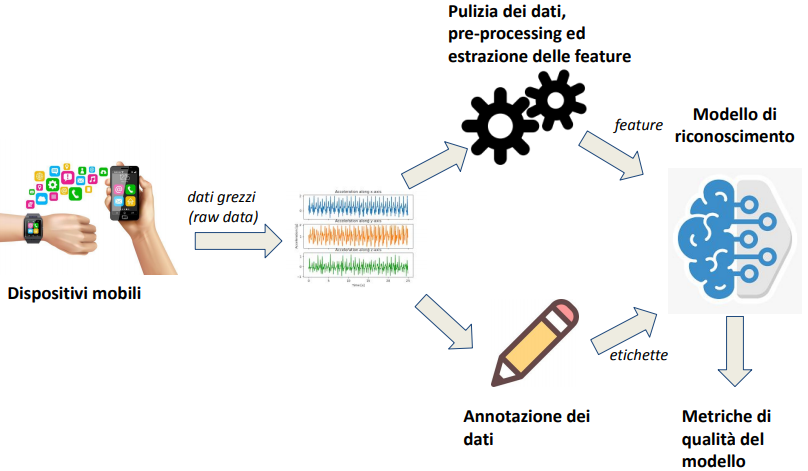
\includegraphics[width=.95\textwidth]{images/MobiDEV/6. activity recognition/addestramento.PNG}
            \caption{fase di addestramento}
            \label{fig:addestramento}
        \end{figure}
    \item riconoscimento: come da figura \ref{fig:riconoscimento}.
\end{itemize} 
Nelle due fasi ci sono passaggi che sono comuni.

\subsubsection{Training set}
Per allenare un algoritmo di riconoscimento è necessario collezionare un dataset etichettato di dati di sensori. È quindi nota la corrispondenza tra dati di sensori e attività. 
È un'operazione molto costosa, e c'è:
\begin{itemize}
    \item la necessità di volontari che svolgono le attività 
    \item la necessità di un’infrastruttura complessa per la raccolta di dati etichettati
\end{itemize} 

Durante la pianificazione del training set è necessario pianificare:
\begin{itemize}
    \item quali attività considerare
    \item quali dispositivi mobili
    \item quante persone coinvolgere
    \item dove svolgere le acquisizioni
    \item decidere se il setting è realistico o guidato
    \item come annotare i dati
    \item quanti minuti di attività acquisire per ogni utente
\end{itemize} 

Le due modalità principali di annotazione dei dati sono:
\begin{itemize}
    \item self annotation: l'attività viene annotata dalla persona stessa, segnando l'inizio e la fine dell'attività. 
    È una modalità intrusiva perché ci possono essere la possibilità di fornire annotazioni sbagliate e svogliatezza nell'annotare
    \item tramite video: si registra ciò che fa una persona tramite dei video e in una seconda fase vengono guardati e i dati vengono annotati. Ci sono problemi di privacy, è soggetto ad errori ed è oneroso in termini di tempo
\end{itemize} 

Una volta effettuate le fasi di acquisizione e annotazione, si hanno a disposizione: 
\begin{itemize}
    \item flussi di dati diversi per ogni sensore, per ogni utente e per i relativi timestamp
    \item informazioni temporali relative all'inizio e alla fine delle attività svolte dagli utenti (etichette)
\end{itemize} 